\let\negmedspace\undefined
\let\negthickspace\undefined
\documentclass[journal]{IEEEtran}
\usepackage[a5paper, margin=10mm, onecolumn]{geometry}
%\usepackage{lmodern} % Ensure lmodern is loaded for pdflatex
\usepackage{tfrupee} % Include tfrupee package

\setlength{\headheight}{1cm} % Set the height of the header box
\setlength{\headsep}{0mm}     % Set the distance between the header box and the top of the text

\usepackage{gvv-book}
\usepackage{gvv}
\usepackage{cite}
\usepackage{amsmath,amssymb,amsfonts,amsthm}
\usepackage{algorithmic}
\usepackage{graphicx}
\usepackage{textcomp}
\usepackage{xcolor}
\usepackage{txfonts}
\usepackage{listings}
\usepackage{enumitem}
\usepackage{mathtools}
\usepackage{gensymb}
\usepackage{comment}
\usepackage[breaklinks=true]{hyperref}
\usepackage{tkz-euclide} 
\usepackage{tikz}
\usepackage{listings}
\usetikzlibrary{patterns}
% \usepackage{gvv}                                        
\def\inputGnumericTable{}                                 
\usepackage[latin1]{inputenc}                                
\usepackage{color}                                            
\usepackage{array}                                            
\usepackage{longtable}                                       
\usepackage{calc}                                             
\usepackage{multirow}                                         
\usepackage{hhline}                                           
\usepackage{ifthen}                                           
\usepackage{lscape}
\begin{document}
\bibliographystyle{IEEEtran}
\vspace{3cm}

\title{GATE\\PH - 2021}
\author{EE24BTECH11061 - Rohith Sai}
\maketitle

\renewcommand{\thefigure}{\theenumi}
\renewcommand{\thetable}{\theenumi}

\section*{General Aptitude (GA)}
\subsection*{Single Correct 1 Mark each}
\begin{enumerate}
\item (i) Arun and Aparna are here.\\
(ii) Arun and Aparna is here.\\
(iii) Arun's families is here.\\
(iv) Arun's family is here.\\
Which of the above sentences are grammatically CORRECT?
\begin{multicols}{2}
    \begin{enumerate}
        \item (i) and (ii)
        \item (i) and (iv)
        \item (ii) and (iv)
        \item (iii) and (iv)
    \end{enumerate}
\end{multicols}

\item \begin{figure}[h!]
    \centering
    \includegraphics[width=0.5\linewidth]{figs/fig.png}
    \caption{Caption}
    \label{fig:enter-label}
\end{figure}
The mirror image of the above text about the x-axis is
\begin{multicols}{2}
    \begin{enumerate}
        \item \includegraphics[width = 0.5\linewidth]{figs/fig_a.jpeg}
        \item \includegraphics[width = 0.5\linewidth]{figs/fig_b.jpeg}
        \item \includegraphics[width = 0.5\linewidth]{figs/fig_c.jpeg}
        \item \includegraphics[width = 0.5\linewidth]{figs/fig_d.jpeg}
    \end{enumerate}
\end{multicols}
    
\item Two identical cube shaped dice each with faces numbered 1 to 6 are rolled simultaneously. The probability that an even number is rolled out on each dice is:
\begin{multicols}{2}
    \begin{enumerate}
        \item $\frac{1}{36}$
        \item $\frac{1}{12}$
        \item $\frac{1}{8}$
        \item $\frac{1}{4}$
    \end{enumerate}
\end{multicols}

\item $\oplus$ and $\odot$ are two operators on numbers $p$ and $q$ such that $p \odot q = p - q$, and $p \odot q = p \times q$\\
Then, $\brak{9 \odot \brak{6 \oplus 7}} \odot \brak{7 \oplus \brak{6 \odot 5}} = $
\begin{multicols}{2}
    \begin{enumerate}
        \item 40
        \item -26
        \item -33
        \item -40
    \end{enumerate}
\end{multicols}

\item Four persons P, Q, R and S are to be seated in row. R should not be seated at the second position from the left end of the row. The number of distinct seating arrangements possible is:
\begin{multicols}{2}
    \begin{enumerate}
        \item 6
        \item 9
        \item 18
        \item 24
    \end{enumerate}
\end{multicols}

\subsection*{Single Correct 2 Marks each}
\item On a planar field, you travelled 3 units East from a point O. Next you travelled 4 units South to arrive at point P. Then you travelled from P in the North-East direction such that you arrive at a point that is 6 units East of point O. Next, you travelled in the North-West direction, so that you arrive at point Q that is 8 units North of point P.\\
The distance of point Q to point O, in the same units, should \rule{1cm}{0.15mm}
\begin{multicols}{2}
    \begin{enumerate}
        \item 3
        \item 4
        \item 5
        \item 6
    \end{enumerate}
\end{multicols}

\item The author said, "Musicians rehearse before their concerts. Actors rehearse their roles before the opening of a new play. On the other hand, I find it strange that many public speakers think they can just walk on to stage and start speaking. In my opinion, it is no less important for public speakers to rehearse their talks."\\
Based on the above passage, which one of the following is TRUE?
\begin{multicols}{2}
    \begin{enumerate}
        \item The author is of the opinion that rehearsing is important for musicians, actors and public speakers.
        \item The author is of the opinion that rehearsing is less important for public speakers than for musicians and actors.
        \item The author is of the opinion that rehearsing is more important only for musicians than public speakers.
        \item The author is of the opinion that rehearsal is more important for actors than musicians.
    \end{enumerate}
\end{multicols}

\item 1. Some football players play cricket.\\
2. All cricket players play hockey.\\
Among the options given below, the statement that logically follows from the two statements 1 and 2 above, is:
\begin{multicols}{2}
    \begin{enumerate}
        \item No football player plays hockey.
        \item Some football players play hockey.
        \item All football players play hockey.
        \item All hockey players play football.
    \end{enumerate}
\end{multicols}

\item \begin{tikzpicture}
    % Define points
    \coordinate (P) at (0, 4);
    \coordinate (Q) at (4, 4);
    \coordinate (R) at (4, 0);
    \coordinate (S) at (0, 0);
    
    % Draw square PQRS
    \draw [thick] (P) -- (Q) -- (R) -- (S) -- cycle;
    
    % Draw quarter circles from P to R
    \draw [thick] (P) arc[start angle=180, end angle=270, radius=4cm];
    \draw [thick] (P) arc[start angle=90, end angle=0, radius=4cm];
    
    % Shading the area between the arcs with lines
    \begin{scope}
        \clip (P) arc[start angle=180, end angle=270, radius=4cm] -- (R) -- (P) arc[start angle=90, end angle=0, radius=4cm] -- cycle;
        \foreach \x in {0.1,0.3,...,3.9} {
            \draw[thin] (\x,0) -- (\x,{sqrt(16-\x*\x)});
        }
    \end{scope}
    
    % Draw radius and arrow
    \draw[thick, ->] (S) -- (2.86,2.86);
    \node at (3,3) {$r$};
    
    % Label points
    \node[above left] at (P) {P};
    \node[above right] at (Q) {Q};
    \node[below right] at (R) {R};
    \node[below left] at (S) {S};
    
    % Label side lengths
    \node[left] at (0,2) {$r$};
    \node[below] at (2,0) {$r$};
    
\end{tikzpicture}
In the figure shown above, PQRS is a square. The shaded portion is formed by the intersection of sectors of circles with radius equal to the side of the square and centers at S and Q.\\
The probability that any point picked randomly within the square falls in the shaded area is \rule{1cm}{0.15mm}
\begin{multicols}{2}
    \begin{enumerate}
        \item $4- \frac{\pi}{2}$
        \item $\frac{1}{2}$
        \item $\frac{\pi}{2} - 1$
        \item $\frac{\pi}{4}$
    \end{enumerate}
\end{multicols}

\item A body flowing in a liquid is in a stable state of equilibrium is its
\begin{multicols}{2}
    \begin{enumerate}
        \item metacentre lies above its centre of gravity
        \item metacentre lies below its centre of gravity
        \item metacentre coincides with its centre of gravity
        \item centre of gravity is below its centre of buoyancy
    \end{enumerate}
\end{multicols}

\item In an equilateral triangle PQR, side PQ is divided into four equal parts, side QR is divided into six equal parts and side PR is divided into eight equal parts.\\
The length of each subdivided part in cm is an integer.\\
The minimum area of the triangle PQR possible, in cm$^2$, is
\begin{multicols}{2}
    \begin{enumerate}
        \item 18
        \item 24
        \item $48 \sqrt{3}$
        \item $144 \sqrt{3}$
    \end{enumerate}
\end{multicols}

\section*{Physics (PH)}
\subsection*{Single Correct 1 Mark each}
\item Choose the graph that best describes the variation of dielectric constant $(\epsilon_r)$ with temperature ($T$) in a ferroelectric material.\\
($T_c$ is the Curie temperature)
\begin{multicols}{2}
    \begin{enumerate}
        \item \begin{tikzpicture}
    % Axes
    \draw[->] (0,0) -- (5,0) node[below] {$T$};
    \draw[->] (0,0) -- (0,3) node[left] {$\epsilon_r$};
    
    % Critical temperature label
    \draw[dashed] (2.5,0) -- (2.5,2.8) node[above] {};
    \node[below] at (2.5,0) {$T_C$};
    
    % Curve with less concavity
    \draw[thick, domain=0:5, samples=100] 
        plot (\x, {2.8 / (1 + 5 * (\x - 2.5)^2)});
    
\end{tikzpicture}

        \item \begin{tikzpicture}
    % Axes
    \draw[->] (0,0) -- (5,0) node[below] {$T$};
    \draw[->] (0,0) -- (0,3) node[left] {$\epsilon_r$};
    
    % Critical temperature label
    \draw[dashed] (2.5,0) -- (2.5,2);
    \node[below] at (2.5,0) {$T_C$};
    
    % Step function
    \draw[thick] (0,2) -- (2.5,2) -- (2.5,1.25);
    \draw[thick] (2.5,1.25) -- (2.5,2);
    
    % Curve after T_C
    \draw[thick] (2.5,1.25) .. controls (3,1) and (4,1) .. (5,2.5);
    
\end{tikzpicture}

        \item \begin{tikzpicture}[scale = 0.7]
    % Axes
    \draw[->] (0,0) -- (5,0) node[right] {$T$};
    \draw[->] (0,0) -- (0,4) node[above] {$\epsilon_r$};

    % Concave curve from origin to T_C, then horizontal line
    \draw[thick, domain=0:2.5, smooth, samples=100] plot (\x, {\x^2 / 2.083});
    \draw[thick] (2.5, 3) -- (4.5, 3);

    % Dotted line for critical temperature
    \draw[dashed] (2.5,0) -- (2.5,3);
    \node at (2.5, -0.5) {$T_C$};
\end{tikzpicture}
        \item \begin{tikzpicture}[scale = 0.7]
    % Axes
    \draw[->] (0,0) -- (5,0) node[right] {$T$};
    \draw[->] (0,0) -- (0,4) node[above] {$\epsilon_r$};

    % Concave decreasing curve
    \draw[thick, domain=0.5:4.5, samples=100, smooth] plot (\x, {1 / (\x)});

    % Dotted line for critical temperature T_C
    \draw[dashed] (2,0) -- (2,2);
    \node at (2,-0.5) {$T_C$};
\end{tikzpicture}
    \end{enumerate}
\end{multicols}

\item A matter wave is represented by the wave function
\begin{align*}
    \psi \brak{x,y,z,t} = A e^{\iota \brak{4x + 3y +5z - 10 \pi t}}
\end{align*}
where A is a constant. The unit vector representing the direction of propagation of this matter wave is
\begin{multicols}{2}
    \begin{enumerate}
        \item $\frac{4}{5\sqrt{2}} \hat{x} + \frac{3}{5\sqrt{2}} \hat{y} + \frac{1}{\sqrt{2}} \hat{z}$
        \item $\frac{3}{5\sqrt{2}} \hat{x} + \frac{4}{5\sqrt{2}} \hat{y} + \frac{1}{5\sqrt{2}} \hat{z}$
        \item $\frac{1}{5\sqrt{2}} \hat{x} + \frac{3}{5\sqrt{2}} \hat{y} + \frac{1}{\sqrt{2}} \hat{z}$
        \item $\frac{1}{5\sqrt{2}} \hat{x} + \frac{4}{5\sqrt{2}} \hat{y} + \frac{3}{5\sqrt{2}} \hat{z}$
    \end{enumerate}
\end{multicols}

\item As shown in figure, X-ray diffraction pattern is obtained from a diatomic chain of atoms P and Q. The diffraction condition is given by $a \cos{\theta} = n \lambda$, where $n$ is the order of the diffraction peak. Here, $a$ is the lattice constant and $\lambda$ is the wavelength of the X-rays. Assume that atomic form factors and resolution of the instrument do not depend on $\theta$. Then, the intensity of the diffraction peaks is
\begin{tikzpicture}

    % Define colors
    \fill[green] (0,0) circle (5pt);
    \node at (0,-0.5) {P};
    \fill[blue] (2,0) circle (5pt);
    \node at (2,-0.5) {Q};
    \fill[green] (4,0) circle (5pt);
    \node at (4,-0.5) {a};
    \fill[blue] (6,0) circle (5pt);
    \fill[green] (8,0) circle (5pt);
    \node at (7,-0.5) {a/2};
    
    % Draw dashed lines for distances
    \draw[dashed] (2,0) -- (4,0);
    \draw[dashed] (8,0.2) -- (8,-0.2);
    
    % Draw the vertical arrows
    \draw[->, red, thick] (2,2) -- (2,1);
    \draw[red, thick] (2,1) -- (2,0);
    \draw[->, red, thick] (2,0) -- (4,2);

    \draw[->, red, thick] (6,2) -- (6,1);
    \draw[red, thick] (6,1) -- (6,0);
    \draw[->, red, thick] (6,0) -- (8,2);

    % Draw angle
    \draw[thick] (2,0) -- (2.5,0) arc[start angle=0, end angle=50, radius=0.5cm];

    % Label the angle
    \node at (2.75,0.3) {$\theta$};
    
    % Draw the horizontal line
    \draw[<->, thick] (2,-0.3) -- (6,-0.3);
    \draw[<->, thick] (6,-0.3) -- (8,-0.3);
\end{tikzpicture}
\begin{multicols}{2}
    \begin{enumerate}
        \item lower for even values of $n$, when compared to odd values of $n$
        \item lower for odd values of $n$, when compared to even values of $n$
        \item zero for odd values of $n$
        \item zero for even values of $n$
    \end{enumerate}
\end{multicols}
\end{enumerate}
\end{document}